\documentclass[12pt,t]{beamer}
\subtitle{02 -- Simple Algorithms}
\newcommand{\shorttitle}{Simple Algorithms}
\usepackage{graphicx}
\setbeameroption{hide notes}
\setbeamertemplate{note page}[plain]

% get rid of junk
\usetheme{default}
\beamertemplatenavigationsymbolsempty
\hypersetup{pdfpagemode=UseNone} % don't show bookmarks on initial view

% font
\usepackage{fontspec}
\setsansfont{TeX Gyre Heros}
\setbeamerfont{note page}{family*=pplx,size=\footnotesize} % Palatino for notes
% "TeX Gyre Heros can be used as a replacement for Helvetica"
% In Unix, unzip the following into ~/.fonts
% In Mac, unzip it, double-click the .otf files, and install using "FontBook"
%   http://www.gust.org.pl/projects/e-foundry/tex-gyre/heros/qhv2.004otf.zip

% named colors
\definecolor{offwhite}{RGB}{249,242,215}
% \definecolor{foreground}{RGB}{255,255,255}
\definecolor{foreground}{RGB}{0,0,0}
% \definecolor{background}{RGB}{24,24,24}
\definecolor{background}{RGB}{255,255,255}
\definecolor{title}{RGB}{107,174,214}
\definecolor{gray}{RGB}{100,100,100}
\definecolor{subtitle}{RGB}{102,155,204}
\definecolor{hilight}{RGB}{20,180,204}
\definecolor{vhilight}{RGB}{255,111,207}
\definecolor{lolight}{RGB}{155,155,155}
%\definecolor{green}{RGB}{125,250,125}

% use those colors
\setbeamercolor{titlelike}{fg=title}
\setbeamercolor{subtitle}{fg=subtitle}
\setbeamercolor{institute}{fg=gray}
\setbeamercolor{normal text}{fg=foreground,bg=background}
\setbeamercolor{item}{fg=foreground} % color of bullets
\setbeamercolor{subitem}{fg=gray}
\setbeamercolor{itemize/enumerate subbody}{fg=gray}
\setbeamertemplate{itemize subitem}{{\textendash}}
\setbeamerfont{itemize/enumerate subbody}{size=\footnotesize}
\setbeamerfont{itemize/enumerate subitem}{size=\footnotesize}

% settings for table of contents
\setbeamercolor{section in toc}{fg=foreground,bg=background}
\setbeamerfont{subsection in toc}{size=\footnotesize}
\setbeamertemplate{section in toc}{{\scriptsize\leavevmode\raise1.35pt\hbox{$\blacktriangleright$}} \inserttocsection}
%\setbeamertemplate{subsection in toc}{\quad{\tiny\leavevmode\raise1.5pt\hbox{$\blacktriangleright$}} \footnotesize\inserttocsubsection\\}
\setbeamertemplate{subsection in toc}{\quad\quad\textendash\enspace\inserttocsubsection\\}

% page number
\setbeamertemplate{footline}{%
    \raisebox{5pt}{\makebox[\paperwidth]{\hfill\makebox[20pt]{\color{gray}
          \scriptsize\insertframenumber}}}\hspace*{5pt}}

% add a bit of space at the top of the notes page
\addtobeamertemplate{note page}{\setlength{\parskip}{12pt}}

% add subsection as frame title when it is empty
\makeatletter
  \CheckCommand*\beamer@checkframetitle{%
    \@ifnextchar\bgroup\beamer@inlineframetitle{}}
  \renewcommand*\beamer@checkframetitle{%
    \global\let\beamer@frametitle\relax\@ifnextchar%
    \bgroup\beamer@inlineframetitle{}}
\makeatother

\addtobeamertemplate{frametitle}{
  \ifx\insertframetitle\empty
      \frametitle{\insertsubsectionhead}
  \else
  \fi
 }{}


\usepackage{pbox}

% a few macros
\newcommand{\bi}{\begin{itemize}}
\newcommand{\ei}{\end{itemize}}
\newcommand{\ig}{\includegraphics}
\newcommand{\subt}[1]{{\footnotesize \color{subtitle} {#1}}}

% title info
\title{Kompetitives Programmieren}
%\author{Gregor Behnke}
\institute{Prof. Dr. Susanne Biundo-Stephan \\ Gregor Behnke \\ Institute of Artificial Intelligence\\ Ulm University}
\date{\tiny based on Bjarki Ágúst Guðmundsson's and Tómas Ken Magnússon's\\Competitive Programming}


\setbeamertemplate{footline}[text line]{%
  \parbox{\linewidth}{\vspace*{-8pt}\shorttitle \hfill \insertframenumber/\inserttotalframenumber}}
\setbeamertemplate{navigation symbols}{}


\newcommand{\specialcell}[2][c]{%
  \begin{tabular}[#1]{@{}c@{}}#2\end{tabular}}

% Tikz
\usepackage{tikz}
\usepackage{tkz-euclide}
\usetikzlibrary{arrows,shapes}
% \usepackage{intersections}
\usetkzobj{all}
\usetikzlibrary{arrows,shapes,angles,quotes,shapes, calc, decorations,matrix}
\usepackage{forest}
\pgfdeclarelayer{bg}    % declare background layer
\pgfsetlayers{bg,main}


% Minted
\usepackage{minted}
\usemintedstyle{tango}
\newminted{cpp}{fontsize=\footnotesize}

% Graph styles
\tikzstyle{vertex}=[circle,fill=black!50,minimum size=15pt,inner sep=0pt, font=\small]
\tikzstyle{selected vertex} = [vertex, fill=red!24]
\tikzstyle{selected2 vertex} = [vertex, fill=hilight!50, text=black]
\tikzstyle{vertex1} = [vertex, fill=red]
\tikzstyle{vertex2} = [vertex, fill=blue]
\tikzstyle{vertex3} = [vertex, fill=green, text=black]
\tikzstyle{vertex4} = [vertex, fill=yellow, text=black]
\tikzstyle{vertex5} = [vertex, fill=pink, text=black]
\tikzstyle{vertex6} = [vertex, fill=purple]
\tikzstyle{edge} = [draw,thick,-]
\tikzstyle{dedge} = [draw,thick,->]
\tikzstyle{weight} = [font=\scriptsize,pos=0.5]
\tikzstyle{selected edge} = [draw,line width=2pt,-,red!50]
\tikzstyle{ignored edge} = [draw,line width=5pt,-,black!20]


\begin{document}

% title slide
{
    \setbeamertemplate{footline}{} % no page number here
    \frame{
        \titlepage
    }
}





\begin{frame}{Today we're going to cover}
    \vspace{30pt}
    \bi
        \item Big Integers
		\item \texttt{set<int>} $\approx$ \texttt{int}
		\item Binary and Ternary Search
		\item 2-Pointer Search
		\item Inversion-Index
        \item Union Find
    \ei
\end{frame}

% \section{Big integers}
% \tableofcontents
\begin{frame}{Big integers}
    \bi
        \item What if we need to represent and do computations with very large integers, i.e.\ something that doesn't fit in a \texttt{long long}
        
        \bi
	  \item C++ has \texttt{\_\_int128\_t}
	\ei

        \vspace{5pt}
        \item Simple ideas
	  \bi
	    \item Store the integer as a string
	    \item Use Java's \texttt{BigInteger}
	  \ei
        \vspace{5pt}
        \item But how do we perform arithmetic on a pair of strings?
        \item We can use the same algorithms as we learned in elementary school
            \bi
                \item Addition: Add digit-by-digit, and maintain the carry
                \item Subtraction: Similar to addition
                \item Multiplication: Long multiplication
                \item Division: Long division
                \item Modulo: Long division
            \ei
        %\item We have a precoded bigint library for C++ %The TCR contains a C++ bigint library
    \ei
\end{frame}

%\begin{frame}{Example problems}
%    \bi
%        \item 424 -- just implement addition or use \texttt{BigInteger}
%        \item 10579 -- Fibonacci
%    \ei
%    
%    There will be more problems in the topics ``Math'' and ``DP''
%\end{frame}


%\begin{frame}{Sorting and searching}
%    \vspace{30pt}
%
%    \bi
%        \item Very common operations:
%            \bi
%                \item Sorting an array \onslide<2->{- {\color{vhilight}sort(all(arr))}}
%                \item Searching an unsorted array \onslide<2->{- {\color{vhilight}find(all(arr), x)}}
%                \item Searching a sorted array \onslide<2->{- {\color{vhilight}lower\_{}bound(all(arr), x)}}
%            \ei
%
%        \item Again, usually in the standard library
%        \item We'll need different versions of binary search later which need custom code, but lower\_{}bound is enough for now
%		    \ei
%\end{frame}
%
%\begin{frame}{Applications of Arrays and Linked Lists}
%    \vspace{40pt}
%    \bi
%        \item Too many to list
%        \item Most problems require storing data, usually in an array
%    \ei
%\end{frame}
%
%\begin{frame}{Example problem: Broken Keyboard}
%    \bi
%        \item http://uva.onlinejudge.org/external/119/11988.html
%    \ei
%\end{frame}
%
%\begin{frame}{Applications of Stacks}
%    \bi
%        \item Processing events in a first-in first-out order
%        \item Simulating recursion
%        \item Depth-first search in a graph
%        \item Reverse a sequence
%        \item Matching brackets
%        \item And a lot more
%    \ei
%\end{frame}
%
%\begin{frame}{Applications of Queues}
%    \bi
%        \item Processing events in a first-in first-out order
%        \item Breadth-first search in a graph
%        \item And a lot more
%    \ei
%\end{frame}
%
%\begin{frame}{Applications of Priority Queues}
%    \bi
%        \item Processing events in order of priority
%        \item Finding a shortest path in a graph
%        \item Some greedy algorithms
%        \item And a lot more
%    \ei
%\end{frame}
%
%\begin{frame}{Applications of Sets}
%    \bi
%        \item Keep track of distinct items
%        \item Have we seen an item before?
%        \item If implemented as a binary search tree:
%            \bi
%        \item Find the successor of an element (the smallest element that is greater than the given element)
%        \item Count how many elements are less than a given element
%        \item Count how many elements are between two given elements
%        \item Find the $k$th largest element
%            \ei
%
%        \item And a lot more
%    \ei
%\end{frame}
%
%\begin{frame}{Applications of Maps}
%    \bi
%        \item Associating a value with a key
%        \item As a frequency table
%        \item As a memory when we're doing Dynamic Programming (later)
%        \item And a lot more
%    \ei
%\end{frame}



\begin{frame}[fragile]{Representing sets}
    \vspace{30pt}
    \bi
        \item We have a small ($n\leq 30$) number of items
        \item We label them with integers in the range $0,1,\ldots,n-1$
        \item We can represent sets of these items as a 32-bit integer
        \item The $i$th item is in the set represented by the integer $x$, if the $i$th bit in $x$ is $1$
        \item Example:
            \bi
                \item We have the set $\{0,3,4\}$
                \item \mint{cpp}.int x = (1<<0) | (1<<3) | (1<<4);.
            \ei
    \ei
\end{frame}

\begin{frame}[fragile]{Representing sets}
    \vspace{5pt}
    \bi
        \item Empty set:
            \mint{cpp}.   0.
        \item Single element set:
            \mint{cpp}.   1<<i.
        \item The universe set (i.e.\ all elements):
            \mint{cpp}.   (1<<n)-1.
        \item Union of sets:
            \mint{cpp}.   x|y.
        \item Intersection of sets: \mint{cpp}.   x&y.
        \item Complement of a set: \mint{cpp}.   ~x & ((1<<n)-1).
    \ei
\end{frame}


\begin{frame}[fragile]{Representing sets}
    \vspace{25pt}
    \bi
        \item Check if an element is in the set:
            \begin{minted}{cpp}

if (x & (1<<i)) {
    // yes
} else {
    // no
}
            \end{minted}
    \ei
\end{frame}

\begin{frame}{Representing sets}
    \vspace{25pt}
    \bi
        \item Why do this instead of using {\color{vhilight}set<int>}?
        \item Very lightweight representation
        \item All subsets of the $n$ elements can be represented by integers in the range $0\ldots 2^{n}-1$
        \item Allows for easily iterating through all subsets (we'll see this later)
        \item Allows for easily using a set as an index of an array (we'll see this later)
    \ei
\end{frame}

\begin{frame}{Binary search}
    \vspace{20pt}
    \bi
        \item We have a \textbf{sorted} array of elements, and we want to check if it contains a particular element $x$
        \vspace{5pt}
        \item Algorithm:
            \begin{enumerate}
                \item Base case: the array is empty, return false
                \item Compare $x$ to the element in the middle of the array
                \item If it's equal, then we found $x$ and we return true
                \item If it's less, then $x$ must be in the left half of the array
                    \begin{enumerate}
                        \item Binary search the element (recursively) in the left half
                    \end{enumerate}
                \item If it's greater, then $x$ must be in the right half of the array
                    \begin{enumerate}
                        \item Binary search the element (recursively) in the right half
                    \end{enumerate}
            \end{enumerate}
    \ei
\end{frame}

\begin{frame}[fragile]{Binary search}
    \vspace{15pt}
    \begin{minted}[fontsize=\scriptsize]{cpp}
bool binary_search(const vector<int> &arr, int lo, int hi, int x) {
    if (lo > hi) {
        return false;
    }

    int m = (lo + hi) / 2;
    if (arr[m] == x) {
        return true;
    } else if (x < arr[m]) {
        return binary_search(arr, lo, m - 1, x);
    } else if (x > arr[m]) {
        return binary_search(arr, m + 1, hi, x);
    }
}

binary_search(arr, 0, arr.size() - 1, x);
    \end{minted}

    \bi
        %\item $T(n) = T(n/2) + 1$
        \item<2-> $O(\log n)$
    \ei
\end{frame}

\begin{frame}[fragile]{Binary search - iterative}
    \vspace{20pt}
    \begin{minted}[fontsize=\scriptsize]{cpp}
bool binary_search(const vector<int> &arr, int x) {
    int lo = 0,
        hi = arr.size() - 1;

    while (lo <= hi) {
        int m = (lo + hi) / 2;
        if (arr[m] == x) {
            return true;
        } else if (x < arr[m]) {
            hi = m - 1;
        } else if (x > arr[m]) {
            lo = m + 1;
        }
    }

    return false;
}
    \end{minted}
\end{frame}

% TODO: Binary search over integers
\begin{frame}{Binary search over integers}
    \bi
        \item This might be the most well known application of binary search, but it's far from being the only application
        \item More generally, we have a predicate $p : \{0,\ldots,n-1\} \rightarrow \{T, F\}$ which has the property that if $p(i) = T$, then $p(j) = T$ for all $j > i$
		\item Further we know that $p(0) = F$ and $p(n-1) = T$
        \item Our goal is to find the smallest index $j$ such that $p(j) = T$ as quickly as possible
    \ei

    \begin{center}
        \begin{tabular}{ccccccccccccccccccc}
            $i$ & $0$ & $1$ & $\cdots$ & $j-1$ & \color{vhilight}{$j$} & $j+1$ & $\cdots$ & $n-2$ & $n-1$ \\
            \hline
            $p(i)$ & $F$ & $F$ & $\cdots$ & $F$ & \color{vhilight}{$T$} & $T$ & $\cdots$ & $T$ & $T$ \\
        \end{tabular}
    \end{center}

    \bi
        \item We can do this in $O(\log(n) \times f)$ time, where $f$ is the cost of evaluating the predicate $p$, in the same way as when we were binary searching an array
    \ei
\end{frame}

\begin{frame}[fragile]{Binary search over integers}
    \begin{minted}[fontsize=\footnotesize]{cpp}
int lo = 0,
    hi = n - 1;

while (lo < hi) {
    int m = (lo + hi) / 2;

    if (p(m)) {
        hi = m;
    } else {
        lo = m + 1;
    }
}
printf("lowest index is %d\n", hi);

    \end{minted}
%if (lo == hi && p(lo)) {
%    printf("lowest index is %d\n", lo);
%} else {
%    printf("no such index\n");
%}
\end{frame}

\begin{frame}[fragile]{Binary search over integers}
    \bi
        \item Find the index of $x$ in the sorted array $arr$
    \ei
    \begin{minted}{cpp}
bool p(int i) {
    return arr[i] >= x;
}
    \end{minted}

		% \vspace{20pt}
    %\bi
    %    \item Later we'll see how to use this in other ways
    %\ei
\end{frame}

% TODO: Binary search over reals
\begin{frame}[fragile]{Binary search over reals}
    \bi
        \item An even more general version of binary search: over real numbers
		\item We have a predicate $p : [lo,hi] \rightarrow \{T, F\}$ which has the property that if $p(i) = T$, then $p(j) = T$ for all $j > i$, also $p(lo)= F$ and $p(hi) = T$
        \item Our goal is to find the smallest real number $j$ such that $p(j) = T$ as quickly as possible

        \vspace{5pt}
        \item Since we're working with real numbers, our $[lo,hi]$ can be halved infinitely many times without ever becoming a single real number
        \item Instead it will suffice to find a real number $j'$ that is very close to the correct answer $j$, say not further than $EPS = 2^{-30}$ away

        \vspace{5pt}
    \item We can do this in $O(\log(\frac{hi - lo}{EPS}) \times f)$ time in a similar way as when we were binary searching an array
    \ei
\end{frame}

\begin{frame}[fragile]{Binary search over reals}
    \begin{minted}{cpp}
double EPS = 1e-10,
       lo = -1000.0,
       hi = 1000.0;

while (hi - lo > EPS) {
    double mid = (lo + hi) / 2.0;

    if (p(mid)) {
        hi = mid;
    } else {
        lo = mid;
    }
}

printf("%0.10lf\n", lo);
    \end{minted}
\end{frame}

\begin{frame}[fragile]{Binary search over reals}
    \bi
        \item This has many cool numerical applications
        \vspace{5pt}
        \item Find the square root of $x$
    \ei
    \begin{minted}{cpp}
bool p(double j) {
    return j*j >= x;
}
    \end{minted}
    \bi
        \item Find the root of an increasing function $f(x)$
    \ei
    \begin{minted}{cpp}
bool p(double x) {
    return f(x) >= 0.0;
}
    \end{minted}

    \bi
        \item This is also referred to as the Bisection method
    \ei
\end{frame}

% TODO: Example problem
%\begin{frame}{Example problem}
%    \bi
%        \item Problem C from NWERC 2006: Pie
%    \ei
%\end{frame}


% TODO: Binary search the answer
\begin{frame}{Binary search the answer}
    \vspace{10pt}
    \bi
        \item It may be hard to find the optimal solution directly
        \item On the other hand, it may be easy to check if some $x$ is a solution or not
        \vspace{5pt}
        \item A method of using binary search to find the minimum or maximum solution to a problem
        \item Only applicable when the problem has the binary search property: if $i$ is a solution, then so are all $j > i$
        \vspace{5pt}
        \item $p(i)$ checks whether $i$ is a solution, then we simply apply binary search on $p$ to get the minimum or maximum solution
    \ei
\end{frame}

\begin{frame}{Ternary Search}
		\bi
%\item Variant of Binary Search, iff $p$ is true only on a single intervall and else false:
%    \begin{center}
%        \begin{tabular}{ccccccccccccccccccc}
%				$i$ & $0$ & $\cdots$ & $j-1$ & \color{vhilight}{$j$} & $\cdots$ & \color{vhilight}{$k$} & $k+1$& $\cdots$ & $n-1$ \\
%            \hline
%				$p(i)$ & $F$ & $\cdots$ & $F$ & \color{vhilight}{$T$} & $\cdots$ & \color{vhilight}{$T$} & $F$ & $\cdots$ & $T$ \\
%        \end{tabular}
%    \end{center}
%		\item We are looking for any
			\item Variant of Binary Search when optimising a convex (or concave) function
			\item Indstead of selecting one point in the middle, divide the current interval in three parts and exclude one of them.
		\ei
		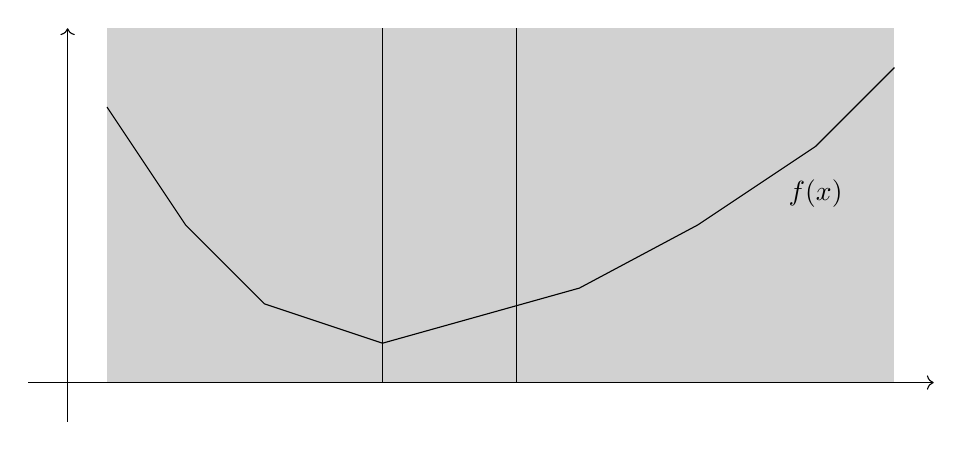
\begin{tikzpicture}

	% 1. step
	\fill<2-3>[gray!30] (-2.5,1.5) -- (-2.5,-3) -- (7.5,-3) -- (7.5,1.5) -- cycle;
	\draw<3> (-2.5+3.3,1.5) -- (-2.5+3.3,-3);
	\draw<3> (7.5-3.3,1.5) -- (7.5-3.3,-3);

	% 2. step
	\fill<4-5>[gray!30] (-2.5,1.5) -- (-2.5,-3) -- (4.2,-3) -- (7.5 - 3.3, 1.5) -- cycle;
	\draw<5> (-2.5 + 2.2, 1.5) -- (-2.5+2.2,-3);
	\draw<5> (4.2-2.2,1.5) -- (4.2-2.2,-3);

	% 3. step
	\fill<6-7>[gray!30] (-0.3,1.5) -- (-0.3,-3) -- (4.2,-3) -- (7.5 - 3.3, 1.5) -- cycle;
	\draw<7> (-0.3 + 1.5, 1.5) -- (-0.3+1.5,-3);
	\draw<7> (4.2-1.5,1.5) -- (4.2-1.5,-3);

	% 4. step
	\fill<8-9>[gray!30] (-0.3,1.5) -- (-0.3,-3) -- (2.7,-3) -- (2.7,1.5) -- cycle;
	\draw<9> (-0.3 + 1.0, 1.5) -- (-0.3+1.0,-3);
	\draw<9> (2.7 - 1.0,1.5) -- (2.7-1.0,-3);

	% 5. step
	\fill<10-11>[gray!30] (-0.3,1.5) -- (-0.3,-3) -- (1.7,-3) -- (1.7,1.5) -- cycle;
	\draw<11> (-0.3 + 0.65, 1.5) -- (-0.3+0.65,-3);
	\draw<11> (1.7 - 0.65,1.5) -- (1.7-0.65,-3);

	% last step
	\fill<12>[gray!30] (0.35,1.5) -- (0.35,-3) -- (1.7,-3) -- (1.7,1.5) -- cycle;
	\draw<13> (1, 1.5) -- (1,-3);

	% fix elements
	\draw<2-> [->] (-3.5,-3) -- (8,-3);
	\draw<2-> [->] (-3,-3.5) -- (-3,1.5);
	\draw<2-> (-2.5,0.5) -- (-1.5,-1) -- (-0.5,-2) -- (1,-2.5) -- (3.5,-1.8) -- (5,-1) -- (6.5,0) -- (7.5,1);
	\node<2-> at (6.5,-0.6) {$f(x)$};
\end{tikzpicture}
\end{frame}



%% TODO: 2-Pointer Search
\begin{frame}{2-Pointer Search}
		\bi
			\item We are given a list of numbers $[a_1, \dots, a_n]$ and a target number $G$.
			\item Find two numbers $a_i$ and $a_j$ s.t. $a_i + a_j \leq G$ and $a_i + a_j$ is maximal
			\vspace{10pt}
			\item<2->Naive Algorithm: Iterate over all pairs and maximise
			\item<2->Problem: the runtime is $\mathcal O(n^2)$
			\vspace{10pt}
			\item<3-> We sort the list and use clever exclusion rules to only test $\mathcal O(n)$ pairs
			\item<3-> Technique is called 2-Pointer Search and is (somehow) related to Sweepline Techniques and Binary Search
		\ei
\end{frame}

\begin{frame}{2-Pointer Search}
    \begin{center}
			$G = 6$\\[1em]
        \begin{tabular}{ccccccc}
				\only<1>{1}\only<2->{0} &
				\only<1>{0}\only<2->{1} &
				\only<1>{7}\only<2->{3} &
				\only<1>{8}\only<2->{4} &
				\only<1>{5}\only<2->{7} &
				\only<1>{9}\only<2->{8} &
				\only<1>{3}\only<2->{9} \\
				\only<3-6>{$\uparrow$}&
				\only<7>{$\uparrow$}&
				\only<8-9>{$\uparrow$}\only<9>{$\uparrow$}&
				\only<6-8>{$\uparrow$}	&
				\only<5>{$\uparrow$}	&
				\only<4>{$\uparrow$}	&
				\only<3>{$\uparrow$}
        \end{tabular}
    \end{center}
\visible<3->{Best Found: }\only<3-5>{none}\only<6>{0 and 4}\only<7-9>{1 and 4}

\end{frame}

\begin{frame}{Inversion Counting}
\bi
	\item Given an array \texttt{a[1..n]} of numbers, how may pairs $i < j$ exists, s.t. \texttt{a[i] > a[j]} ?
	\vspace{10pt}
	\item<2-> Naive approach: iterate and test
	\item<2-> Problem: the runtime is $\mathcal O(n^2)$
	\vspace{10pt}
	\item<3-> Use Mergesort!
	\item<3-> Run Mergesort as ususal. If at a merge-comparison, the number in the left subarray is bigger than the one in the right, we have found inversion\textbf{s}!
	\item<4-> How many?
	\item<5-> As many as numbers are remain in the left subarray!
\ei
\end{frame}

\begin{frame}[fragile]{Inversion Counting}
    \begin{minted}[fontsize=\tiny]{cpp}
int  _mergeSort(int arr[], int temp[], int left, int right);
int merge(int arr[], int temp[], int left, int mid, int right);
 
int mergeSort(int arr[], int array_size){
    int *temp = (int *)malloc(sizeof(int)*array_size);
    return _mergeSort(arr, temp, 0, array_size - 1);
}
 
int _mergeSort(int arr[], int temp[], int left, int right)
{
  int mid, inv_count = 0;
  if (right > left)  {
    mid = (right + left)/2;
    inv_count  = _mergeSort(arr, temp, left, mid);
    inv_count += _mergeSort(arr, temp, mid+1, right);
    inv_count += merge(arr, temp, left, mid+1, right);
  }
  return inv_count;
}
 
int merge(int arr[], int temp[], int left, int mid, int right){
  int i = left, j = mid, k = left, inv_count = 0;
  while ((i <= mid - 1) && (j <= right)) {
    if (arr[i] <= arr[j]) temp[k++] = arr[i++];
    else temp[k++] = arr[j++], inv_count = inv_count + (mid - i);
    }
  }
  while (i <= mid - 1) temp[k++] = arr[i++]; 
  while (j <= right) temp[k++] = arr[j++];
  for (i=left; i <= right; i++) arr[i] = temp[i];
  return inv_count;
}
	\end{minted}

\end{frame}


% TODO: Union-Find
\begin{frame}[fragile]{Union-Find}
    \vspace{20pt}
    \bi
        \item We have $n$ items
        \item Maintains a collection of disjoint sets
        \item Each of the $n$ items is in exactly one set
        \vspace{10pt}
        \item $items = \{1,2,3,4,5,6\}$
        \item $collections = \{1,4\}, \{3,5,6\}, \{2\}$
        \item $collections = \{1\}, \{2\}, \{3\}, \{4\}, \{5\}, \{6\}$
        \vspace{10pt}
        \item Supports two operations efficiently: \texttt{find(x)} and \texttt{union(x,y)}.
    \ei
\end{frame}

\begin{frame}{Union-Find}
    \bi
        \vspace{10pt}
        \item $items = \{1,2,3,4,5,6\}$
        \item $collections = \{1,4\}, \{3,5,6\}, \{2\}$
        \vspace{10pt}
        \item \texttt{find(x)} returns a representative item from the set that $x$ is in
            \bi
                \vspace{5pt}
                \item \texttt{find(1) = 1}
                \item \texttt{find(4) = 1}
                \vspace{5pt}
                \item \texttt{find(3) = 5}
                \item \texttt{find(5) = 5}
                \item \texttt{find(6) = 5}
                \vspace{5pt}
                \item \texttt{find(2) = 2}
            \ei
        \vspace{5pt}
        \item $a$ and $b$ are in the same set if and only if \\ \texttt{find(a) == find(b)}
    \ei
\end{frame}

\begin{frame}{Union-Find}
    \bi
        \vspace{10pt}
        \item $items = \{1,2,3,4,5,6\}$
        \item $collections = \{1,4\}, \{3,5,6\}, \{2\}$
        \vspace{10pt}
        \item \texttt{union(x, y)} merges the set containing $x$ and the set containing $y$ together.
        \vspace{10pt}
            \bi
                \item \texttt{union(4, 2)}
                \item $collections = \{1,2,4\}, \{3,5,6\}$
                \item \texttt{union(3, 6)}
                \item $collections = \{1,2,4\}, \{3,5,6\}$
                \item \texttt{union(2, 6)}
                \item $collections = \{1,2,3,4,5,6\}$
            \ei
    \ei
\end{frame}

\begin{frame}[fragile]{Union-Find implementation}
    \bi
        \item Quick Union with path compression
        \item Extremely simple implementation
        \item Extremely efficient
    \ei

    \vspace{10pt}

    \begin{minted}{cpp}
int pa[MAXN];
int rk[MAXN];

int ufind(int i) {
    if(pa[i] != i) pa[i] = ufind(pa[i]);
    return pa[i];
}
    \end{minted}
\end{frame}

\begin{frame}[fragile]{Union-Find implementation}

    \begin{minted}{cpp}
int pa[MAXN];
int rk[MAXN];

int uunion(int a,int b) {
    a = ufind(a); b = ufind(b);
    if(a == b) return 0;
    if(rk[a] > rk[b])
        pa[b] =a;
    else
        pa[a] = b;
    if(rk[a] == rk[b]) rk[b]++;
    return 1;
}
    \end{minted}
		\bi
\item<2-> Runtime? \visible<3->{$\mathcal O(\log^* n)$} \visible<4-> {aka $ \leq 5$ for $n < 2^{2^{16}}$}
		\ei
\end{frame}

\begin{frame}[fragile]{Union-Find implementation (short)}
    \bi
        \item If you're in a hurry...
    \ei

\vspace{20pt}

    \begin{minted}{cpp}
#define MAXN 1000
int p[MAXN];

int find(int x) {
    return p[x] == x ? x : p[x] = find(p[x]); }
void unite(int x, int y) { p[find(x)] = find(y); }

FOR(i,0,n) p[i] = i;
    \end{minted}
\end{frame}

\begin{frame}{Union-Find applications}
    \vspace{30pt}
    \bi
        \item Union-Find maintains a collection of disjoint sets
        \item When are we dealing with such collections?
        \item Most common example is in graphs
    \ei
\end{frame}

\begin{frame}{Disjoint sets in graphs}
    \begin{figure}
        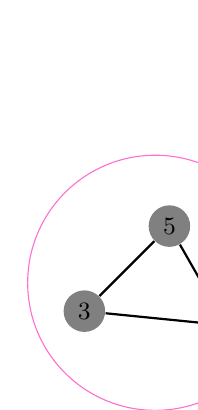
\begin{tikzpicture}[scale=1.8,auto,swap]

            \node[vertex] (1) at (-0.8,1.9) {1};
            \node[vertex] (2) at (3,1.7) {2};
            \node[vertex] (3) at (0.4,0.5) {3};
            \node[vertex] (4) at (-1.2,1.2) {4};
            \node[vertex] (5) at (1,1.1) {5};
            \node[vertex] (6) at (1.4,0.4) {6};
            \node[vertex] (7) at (-1.9,1.7) {7};

            \path[edge] (1) -- (4);
            \path[edge] (4) -- (7);
            \path[edge] (3) -- (5);
            \path[edge] (5) -- (6);
            \path[edge] (6) -- (3);

            \onslide<3->{
                \draw[color=vhilight] (-1.3,1.55) ellipse (0.9cm and 0.9cm);
                \draw[color=vhilight] (0.9,0.7) ellipse (0.9cm and 0.9cm);
                \draw[color=vhilight] (3,1.7) ellipse (0.3cm and 0.3cm);
            }

            \pgfresetboundingbox
            \path [use as bounding box] (0,0) rectangle (1,2.5);
        \end{tikzpicture}
    \end{figure}

    \bi
        \onslide<2->{\item $items = \{1,2,3,4,5,6,7\}$}
        \onslide<3->{\item $collections = \{1,4,7\}, \{2\}, \{3,5,6\}$}
        \onslide<4->{\item \texttt{union(2, 5)}}
    \ei
\end{frame}


\begin{frame}{Disjoint sets in graphs}
    \begin{figure}
        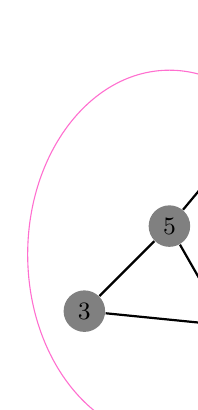
\begin{tikzpicture}[scale=1.8,auto,swap]

            \node[vertex] (1) at (-0.8,1.9) {1};
            \node[vertex] (2) at (1.5,1.7) {2};
            \node[vertex] (3) at (0.4,0.5) {3};
            \node[vertex] (4) at (-1.2,1.2) {4};
            \node[vertex] (5) at (1,1.1) {5};
            \node[vertex] (6) at (1.4,0.4) {6};
            \node[vertex] (7) at (-1.9,1.7) {7};

            \path[edge] (1) -- (4);
            \path[edge] (4) -- (7);
            \path[edge] (3) -- (5);
            \path[edge] (5) -- (6);
            \path[edge] (6) -- (3);
            \path[edge] (2) -- (5);

            \draw[color=vhilight] (-1.3,1.55) ellipse (0.9cm and 0.9cm);
            \draw[color=vhilight] (1.0,0.9) ellipse (1.0cm and 1.3cm);

            \pgfresetboundingbox
            \path [use as bounding box] (0,0) rectangle (1,2.5);
        \end{tikzpicture}
    \end{figure}

    \bi
        \item $items = \{1,2,3,4,5,6,7\}$
        \item $collections = \{1,4,7\}, \{2,3,5,6\}$
        \onslide<2->{\item \texttt{union(6, 2)}}
    \ei
\end{frame}


\begin{frame}{Disjoint sets in graphs}
    \begin{figure}
        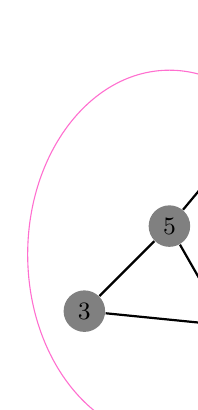
\begin{tikzpicture}[scale=1.8,auto,swap]

            \node[vertex] (1) at (-0.8,1.9) {1};
            \node[vertex] (2) at (1.5,1.7) {2};
            \node[vertex] (3) at (0.4,0.5) {3};
            \node[vertex] (4) at (-1.2,1.2) {4};
            \node[vertex] (5) at (1,1.1) {5};
            \node[vertex] (6) at (1.4,0.4) {6};
            \node[vertex] (7) at (-1.9,1.7) {7};

            \path[edge] (1) -- (4);
            \path[edge] (4) -- (7);
            \path[edge] (3) -- (5);
            \path[edge] (5) -- (6);
            \path[edge] (6) -- (3);
            \path[edge] (2) -- (5);
            \path[edge] (2) -- (6);

            \draw[color=vhilight] (-1.3,1.55) ellipse (0.9cm and 0.9cm);
            \draw[color=vhilight] (1.0,0.9) ellipse (1.0cm and 1.3cm);

            \pgfresetboundingbox
            \path [use as bounding box] (0,0) rectangle (1,2.5);
        \end{tikzpicture}
    \end{figure}

    \bi
        \item $items = \{1,2,3,4,5,6,7\}$
        \item $collections = \{1,4,7\}, \{2,3,5,6\}$
    \ei
\end{frame}





\end{document}
